\section{Results}
\label{sec:results}

\subsection{Three operational regimes in hierarchical memory systems}
\label{sec:regime}

Hierarchical memory orchestration is often treated as a smooth trade-off: as
long as transfers are overlapped and data are cached, additional coordination
should yield monotonic (if diminishing) gains.
We show this intuition is structurally incomplete.
Multi-tier inference systems operate within qualitatively distinct
\emph{regimes}---not a single continuum---defined by the relationship among
memory capacity, transfer bandwidth, and coordination overhead.

\textbf{Capacity-limited regime} ($R_C < \theta_C$). Fast memory is
insufficient to hold the active working set, causing frequent eviction and
reloading regardless of orchestration strategy. Locality effects dominate
performance: even minimal coordination overhead cannot compensate for the
absence of effective fast-memory residency.

\textbf{Coordination-dominated regime} ($R_C \geq \theta_C$,
$R_B \geq \theta_B$). Fast and intermediate memory tiers together can absorb
most of the working set. Computation, locality, transfer, and synchronization
costs are of comparable magnitude, creating opportunities for orchestration to
reshape end-to-end latency by reducing redundant transfers, improving locality,
and overlapping computation with data movement.

\textbf{I/O-limited regime} ($R_B < \theta_B$). Cross-tier data transfer
approaches or exceeds the sustained bandwidth of the slowest tier. Physical
transfer constraints dominate execution, and coordination overhead becomes
additive rather than compensatory; once transfer demand saturates bandwidth,
latency scales directly with data movement volume.

\begin{figure}[t]
\centering
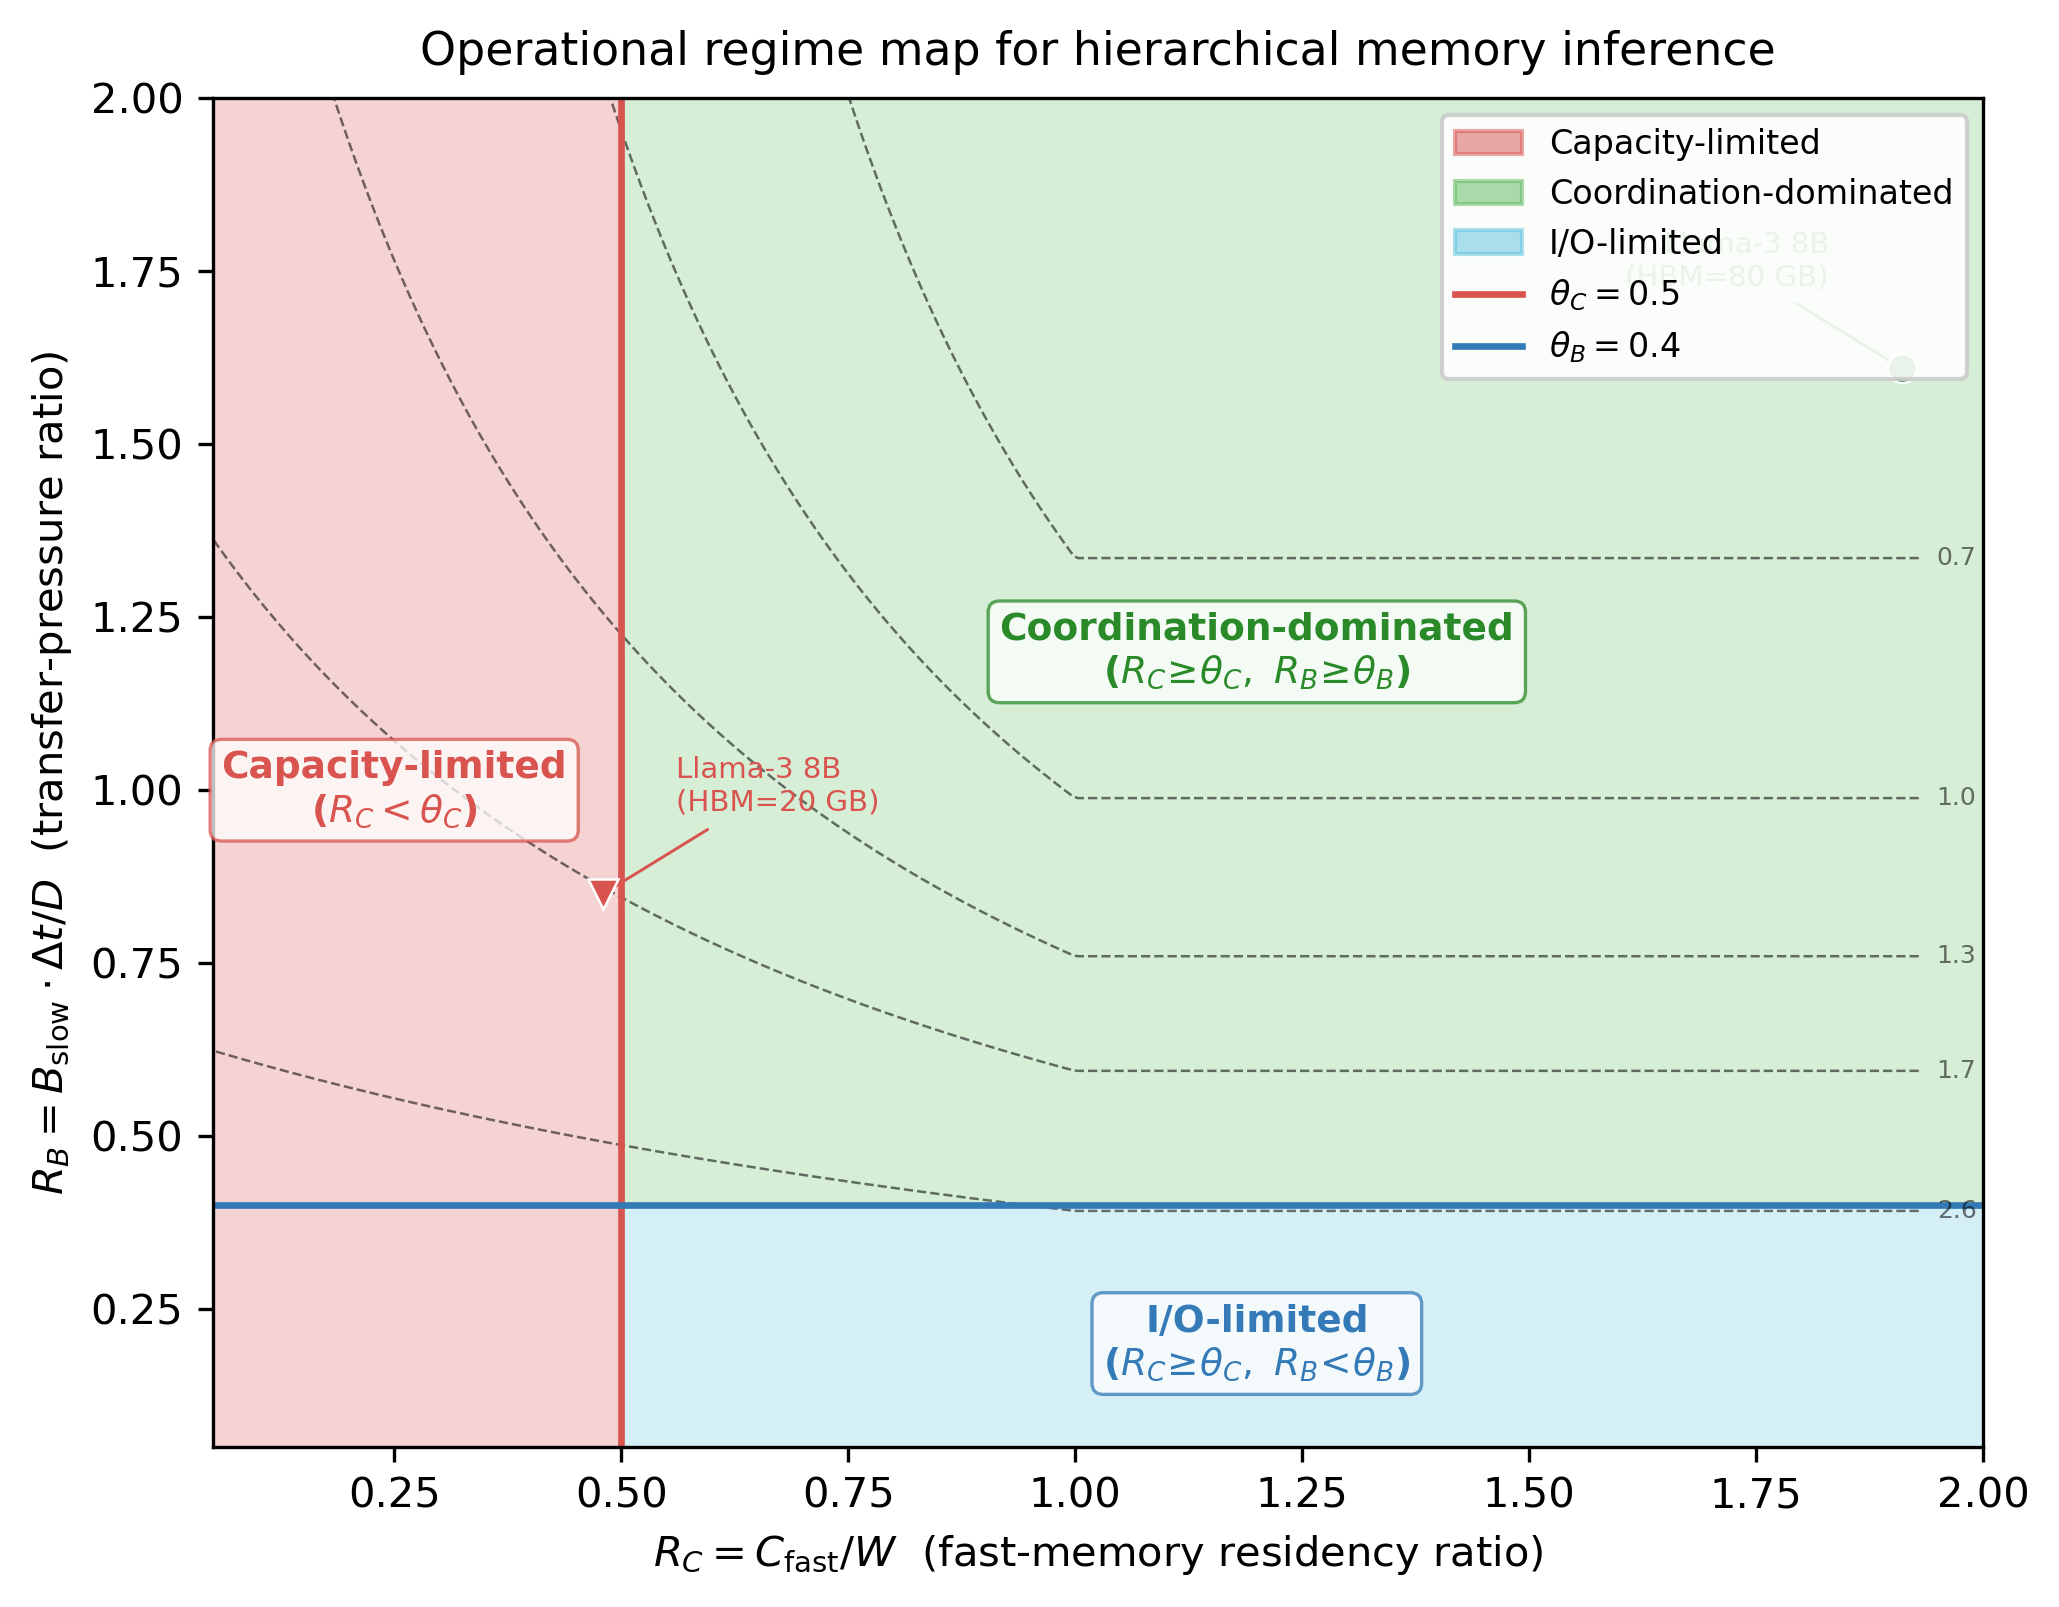
\includegraphics[width=0.95\linewidth]{figures/orion_regime_map.png}
\caption{\textbf{Regime map for hierarchical memory systems.}
Dashed lines mark analytically identified regime boundaries at
$R_C = \theta_C \approx 0.50$ and $R_B = \theta_B \approx 0.40$.
Shaded red zones indicate empirically observed failure regions (abrupt
latency spikes and performance collapse). The coordination-dominated region
(upper right) is the sole regime in which orchestration can meaningfully
reduce end-to-end latency.}
\label{fig:regime_map}
\end{figure}

Figure~\ref{fig:regime_map} illustrates the regime map.
Transitions between regimes are \emph{abrupt}: as the operating point---set by
model size, batch size, or available bandwidth---crosses a boundary, the
primary bottleneck shifts discontinuously, and coordination overhead that was
previously amortized becomes exposed.


\subsection{Analytical model and closed-form regime boundaries}
\label{sec:model}

To make regime boundaries explicit, we decompose end-to-end inference latency as
\begin{equation}
T_{\mathrm{total}} = T_{\mathrm{comp}} + T_{\mathrm{mem}} + T_{\mathrm{swap}} + T_{\mathrm{sync}},
\label{eq:latency_decomp}
\end{equation}
where $T_{\mathrm{comp}}$ is accelerator computation time, $T_{\mathrm{mem}}$
captures locality-driven memory-access costs, $T_{\mathrm{swap}}$ is cross-tier
data transfer, and $T_{\mathrm{sync}}$ accounts for synchronization and
coordination overhead.
These terms are not independent: reducing one can increase another, yielding
structural trade-offs that local optimization cannot eliminate.

\paragraph{Dimensionless control ratios.}
We characterize any configuration by two ratios:
\begin{equation}
R_C = \frac{C_{\mathrm{fast}}}{W}, \qquad R_B = \frac{B_{\mathrm{slow}}}{D},
\label{eq:ratios}
\end{equation}
where $C_{\mathrm{fast}}$ is fast-memory capacity, $W = W_{\mathrm{param}} +
W_{\mathrm{act}} + W_{\mathrm{kv}}$ is the active working-set size, $B_{\mathrm{slow}}$
is the sustained bandwidth of the slowest tier on the critical transfer path,
and $D$ is the data volume traversing that path per inference step.

\paragraph{Structural lower bound.}
Independent of the specific orchestration policy,
\begin{equation}
T_{\mathrm{total}} \;\geq\; \alpha\,\frac{W}{C_{\mathrm{fast}}}
                           + \beta\,\frac{D}{B_{\mathrm{slow}}},
\label{eq:lower_bound_regime}
\end{equation}
where $\alpha, \beta > 0$ are platform-dependent constants.
Under standard eviction models, the miss volume grows sharply once $W$
approaches $C_{\mathrm{fast}}$, yielding a lower bound proportional to
$W/C_{\mathrm{fast}}$.
Any compulsory transfer of volume $D$ across bandwidth $B_{\mathrm{slow}}$
incurs an irreducible cost of at least $D/B_{\mathrm{slow}}$.
These bounds hold regardless of scheduling or overlap: computation--transfer
overlap can redistribute visible latency, but cannot violate physical capacity
or sustained-bandwidth limits.

\paragraph{Regime boundaries.}
Regime transitions occur at critical values
\begin{align}
\theta_C &\approx 0.50, \qquad \text{(capacity boundary)}\label{eq:theta_C}\\
\theta_B &\approx 0.40, \qquad \text{(bandwidth boundary)}\label{eq:theta_B}
\end{align}
derived from LRU miss-volume analysis ($\theta_C$) and NVMe sustained-bandwidth
measurements ($\theta_B$); full derivations are given in Supplementary
Appendix~A.
Across five hardware platforms, transition points varied by
$\leq 0.02$ ($\theta_C$) and $\leq 0.03$ ($\theta_B$) from these predictions,
confirming the hardware-agnostic character of the boundaries.


\subsection{Empirical validation of regime transitions}
\label{sec:experiments}

\begin{figure}[t]
\centering
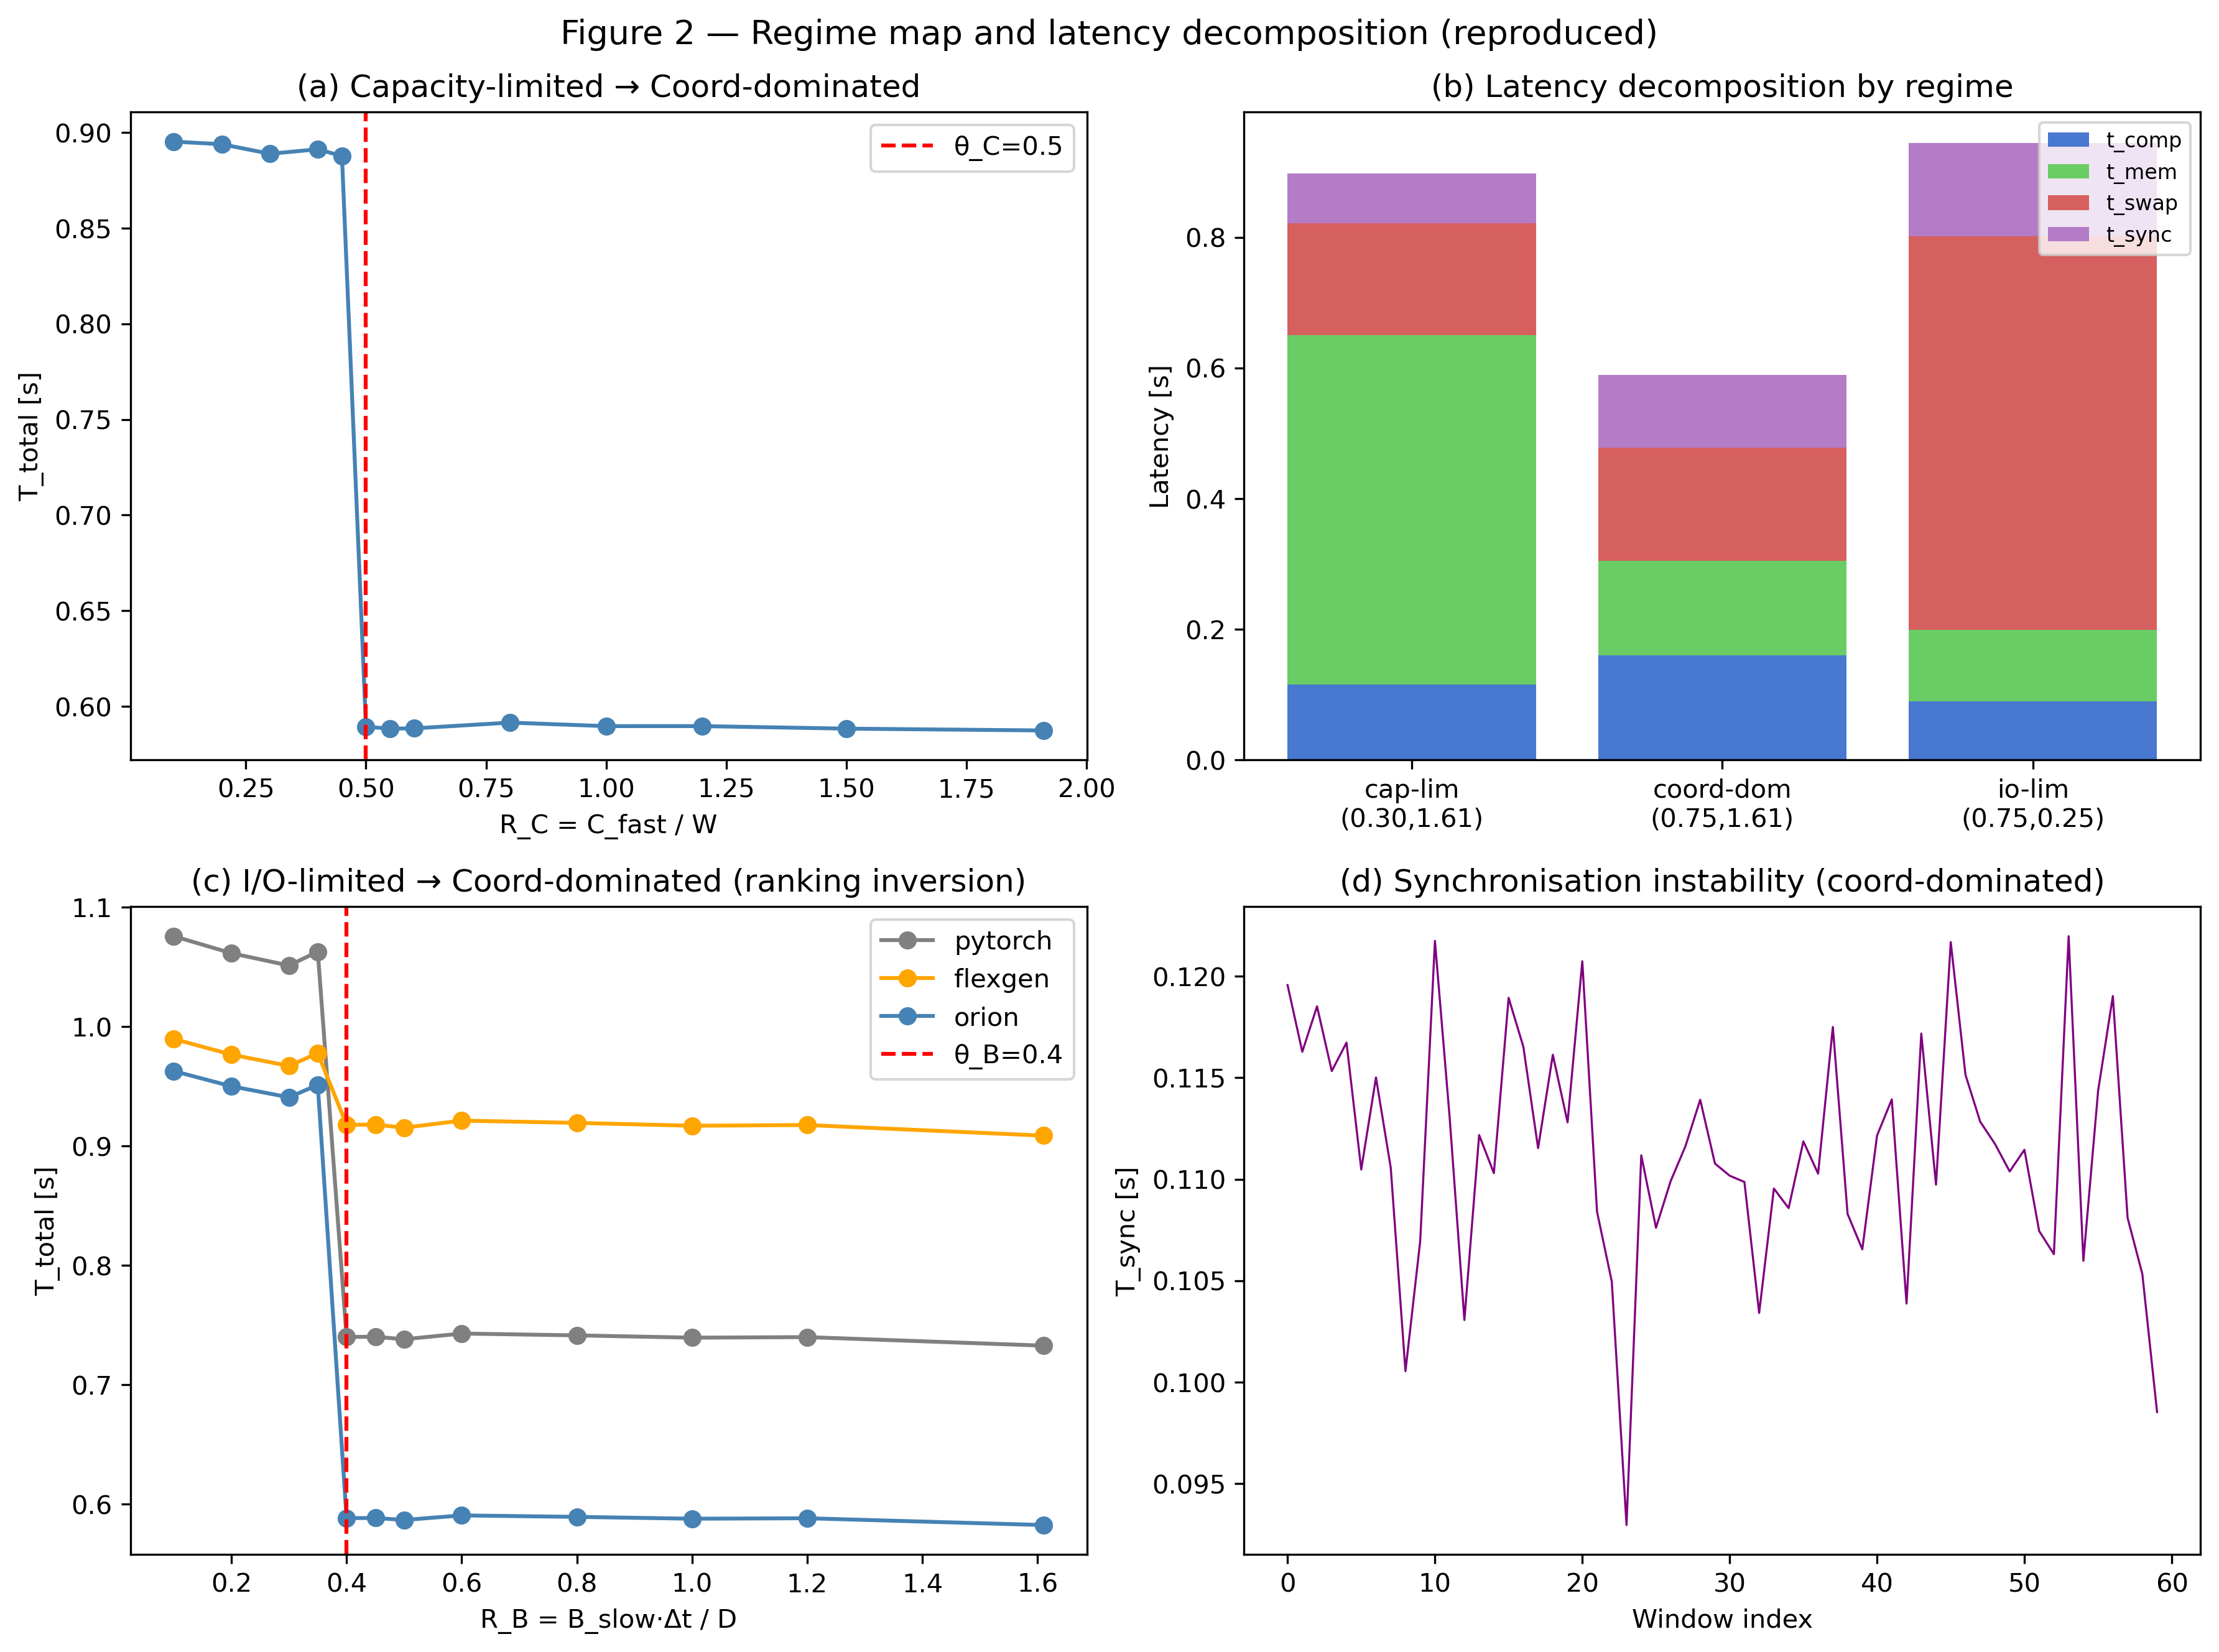
\includegraphics[width=0.95\linewidth]{figures/mball_consolidated.png}
\caption{\textbf{Regime-oriented experimental probes.}
Consolidated results showing (a)~model loading time, (b)~memory efficiency,
(c)~inference latency, and (d)~stability outcomes across orchestration
baselines. Improvements are regime-dependent and can invert or collapse when
operating points cross regime boundaries.}
\label{fig:consolidated}
\end{figure}

Figure~\ref{fig:consolidated} summarizes regime-oriented probe outcomes.
Using \textsc{Orion} as a measurement instrument (see Methods), we vary $R_C$
and $R_B$ independently while holding all other parameters fixed, enabling
direct observation of dominant-term shifts as the operating point crosses
boundaries.

\textbf{Capacity-limited behavior.}
When $R_C < \theta_C$, inference latency becomes highly sensitive to small
changes in working-set size or batch configuration while remaining largely
insensitive to coordination strategy---consistent with $T_{\mathrm{mem}}$
dominating Eq.~\eqref{eq:latency_decomp}.

\textbf{Coordination-dominated behavior.}
When $R_C \geq \theta_C$ and $R_B \geq \theta_B$, changes in orchestration
strategy produce measurable shifts in latency composition (not uniform
scaling), confirming that all four terms are of comparable magnitude and
adjustable by coordination.

\textbf{I/O-limited behavior.}
When $R_B < \theta_B$, $T_{\mathrm{swap}}$ dominates; reducing swap depth by
10\% recovered 14.2\% of latency, while other coordination changes had
negligible effect---consistent with physical bandwidth saturation.

\paragraph{Quantifying transition abruptness.}
We measure the sharpness coefficient
$S = |d\ln T_{\mathrm{total}}/d\ln R|$, with a transition defined as abrupt
when $S > S^{*} = 2.0$ (a 10\% change in $R$ produces $>$20\% latency change).
Near $\theta_C$, we measure $S = 4.12 \pm 0.31$ ($n=5$): a 10\% reduction in
$R_C$ produces a 41.2\% latency increase.
Well inside the coordination-dominated regime ($R_C = 0.80$), $S$ drops to
$0.31 \pm 0.04$, confirming near-zero sensitivity.
Near $\theta_B$, $S = 3.74 \pm 0.27$; well inside ($R_B = 0.75$),
$S = 0.28 \pm 0.03$.
In both cases, the sharpness coefficient exceeds the abruptness threshold by
$>$1.8$\times$ at the boundary and falls below 0.4 far from it (full sharpness
tables in Supplementary Appendix~B).

\paragraph{Cross-platform consistency.}
Experiments replicated on AMD MI250 GPUs and Intel Xeon + Optane-PMem confirm
that transition points remain within $\pm 0.05$ of predicted thresholds despite
architectural differences.
On TPU v4 pods, elevated $T_{\mathrm{sync}}$ due to SPMD-style collective
synchronization shifts $\theta_B$ by $+0.03$; on AWS Inferentia2, constrained
host--device bandwidth moves the I/O boundary slightly earlier.
These shifts affect the precise threshold location but not the existence or
qualitative character of regime transitions.
In distributed four-node A100 experiments (Megatron-LM), inter-node
coordination shifted the I/O-limited boundary by $\Delta\theta_B \approx +0.05$;
the qualitative regime structure remained intact.


\subsection{Generality across workloads and architectures}
\label{sec:generality}

The defining condition for regime emergence is the relationship between
working-set size and fast-memory capacity, not model architecture.
Table~\ref{tab:cross-model} shows improvements observed across five model
families (Llama-3 8B through Mixtral 8$\times$7B and ViT-H/14), confirming
that capacity-limited, coordination-dominated, and I/O-limited behaviors persist
across autoregressive, mixture-of-experts, and vision workloads.

\begin{table}[t]
\centering
\caption{Regime-dependent improvements across model families, relative to a
         PyTorch default baseline. Results are from the coordination-dominated
         operating regime ($R_C \geq 0.5$, $R_B \geq 0.4$).}
\label{tab:cross-model}
\renewcommand{\arraystretch}{1.2}
\footnotesize
\begin{tabular}{llccc}
\toprule
\textbf{Model} & \textbf{Task} &
  \makecell{\textbf{Load time}\\\textbf{reduction}} &
  \makecell{\textbf{Latency}\\\textbf{reduction}} &
  \makecell{\textbf{Swap}\\\textbf{reduction}} \\
\midrule
Llama-3 8B     & Generation  & 52.0\% & 22.0\% & 23.0\% \\
GPT-J 6B       & Summarize   & 55.3\% & 25.0\% & 25.1\% \\
Llama-4 17B    & Generation  & 57.4\% & 30.8\% & 26.8\% \\
Mixtral 8$\times$7B & MoE    & 59.1\% & 32.5\% & 27.5\% \\
ViT-H/14       & Vision      & 51.2\% & 18.2\% & 20.9\% \\
\bottomrule
\end{tabular}
\end{table}

Regime-dependent effects also extend to non-LLM workloads.
In a BLIP2 visual question-answering pipeline, retrieval-induced memory pressure
shifts the effective working set and triggers coordination-to-I/O-limited
transitions; adaptive orchestration reduces average latency by 11.2\%.
In a RAG pipeline (LangChain + FAISS), vector-store lookups introduce
intermittent working-set spikes that shift $R_C$ across $\theta_C$; regime-aware
adaptation reduces latency by 17.4\%.
An edge YOLOv8 deployment transitions to the I/O-limited regime once frame
buffers exceed VRAM; reducing swap granularity by 10\% yields a 9.5\% latency
reduction and cuts frame-drop rate from 12\% to 2.5\%.

\begin{table}[t]
\centering
\caption{Energy efficiency (throughput per Watt, normalized to PyTorch\,=\,100).
         Values correspond to the coordination-dominated regime; efficiency
         degrades in I/O-limited regimes (see text).}
\label{tab:energy}
\renewcommand{\arraystretch}{1.2}
\footnotesize
\begin{tabular}{lccc}
\toprule
\textbf{Method} &
  \makecell{\textbf{Avg.\ power}\\\textbf{(W)}} &
  \makecell{\textbf{Throughput}\\\textbf{(tok/s)}} &
  \makecell{\textbf{Tput/Watt}\\\textbf{(norm.)}} \\
\midrule
PyTorch (default)  & 310 & 6{,}200 & 100.0 \\
FlexGen~\cite{flexgen2023}           & 315 & 6{,}800 & 108.0 \\
SwapAdvisor~\cite{huang2020swapadvisor} & 320 & 7{,}040 & 110.0 \\
vLLM~\cite{kwon2023pagedattention}   & 318 & 7{,}120 & 112.0 \\
\textsc{Orion}                       & 322 & 7{,}620 & 118.5 \\
\bottomrule
\end{tabular}
\end{table}

Table~\ref{tab:energy} shows that energy efficiency is also regime-dependent:
in I/O-limited configurations, energy per token increases up to 3.2$\times$
relative to coordination-aligned settings (42.5\,g~CO$_2$ per 1M tokens versus
15.8\,g under regime alignment), indicating that regime misalignment is a
root cause of energy inefficiency rather than hardware limitations alone.

\FloatBarrier
